\documentclass[10pt,a4paper]{beamer}
\usepackage[utf8]{inputenc}
\usepackage[T1]{fontenc}
\usepackage[english]{babel}
\usepackage{hyperref}
\usepackage{amssymb,amsthm,amsmath,amsfonts}
\usepackage{lmodern}
\usepackage{units}
\usepackage{hyperref}
\usepackage{tikz}
\usepackage{tikzsymbols}
\usetikzlibrary{calc}
\usetikzlibrary{fixedpointarithmetic}
\usepackage{fp}
\usepackage{graphicx}
\bibliographystyle{plain}
\usepackage{epsfig}
\usepackage{epstopdf}
\usepackage{makeidx}
\usepackage{gloss}
\usepackage{algorithmic}
\usepackage{algorithm}

\usepackage{xkeyval} 

\def\glossname{Glossaire}
%\bibliographystyle{alpha} % plain-fr si rapport en français

\usepackage[usenames,dvipsnames]{pstricks}
\usepackage{epsfig}
\usepackage{pst-grad} % For gradients
\usepackage{pst-plot}



\theoremstyle{plain}
\newtheorem{thm}{Theorem}[part]
\theoremstyle{definition} 
\newtheorem{lem}[thm]{Lemma}
\theoremstyle{definition} 
\newtheorem{cor}[thm]{Corollary}
\theoremstyle{definition} 
\newtheorem{prop}[thm]{Proposition}
\theoremstyle{definition} 
\newtheorem{defi}[thm]{Definition}
\theoremstyle{remark} 
\newtheorem{rem}[thm]{Remark}
\theoremstyle{remark} 
\newtheorem{exe}[thm]{Example}

\useoutertheme{split}
\useinnertheme{rounded}
\usecolortheme{whale}
\usecolortheme{orchid}
\usecolortheme[named=orange]{structure}
\definecolor{pacificcream}{cmyk}{.05,.05,.15,0}


\setbeamerfont{block title}{size={}}
\beamertemplatenavigationsymbolsempty

\newcommand{\orangebox}[2]{
\setbeamercolor{uppercol}{fg=white,bg=orange}
\setbeamercolor{lowercol}{fg=black,bg=pacificcream}

\begin{beamerboxesrounded}[upper=uppercol,lower=lowercol,shadow=true]{
#1 }  #2
\end{beamerboxesrounded} }

\newcommand{\bluebox}[2]{
\setbeamercolor{upperblue}{fg=white,bg=blue}
\setbeamercolor{lowercol}{fg=black,bg=pacificcream}

\begin{beamerboxesrounded}[upper=upperblue,lower=lowercol,shadow=true]{
#1 }  #2
\end{beamerboxesrounded} }

\newenvironment{orangeitemize}{\setbeamertemplate{itemize item}{$\bullet$}\begin{itemize}}{\end{itemize}}
\newenvironment{grassgreenitemize}{\setbeamertemplate{itemize item}{\textcolor{grassgreen}{$\bullet$}} \begin{itemize}}{\end{itemize}}
\newenvironment{blackitemize}{\setbeamertemplate{itemize item}{\textcolor{black}{$\bullet$}} \begin{itemize}}{\end{itemize}}


\logo{
\includegraphics[height=8mm]{Images/uvsq-logo-cmjn.jpg}} 
\addtobeamertemplate{footline}{\hfill\insertframenumber/ \inserttotalframenumber \hspace{2em}\null}

\def\algorithmicrequire{\textbf{Input:}}
\def\algorithmicensure{\textbf{Output:}}

\def\red#1{\textcolor{red}{#1}}
\def\blu#1{\textcolor{blue}{#1}}

\begin{document}

\author{
 Luca De Feo, \underline{Cyril Hugounenq}, J\'er\^ome Pl\^ut, \'Eric Schost
}
%\title[Structure of $\ell$-isogeny volcanoes applied to Couveignes' algorithm]{Structure of $\ell$-isogeny volcanoes applied to Couveignes' algorithm}
\title[Explicit isogenies in quadratic time in any characteristic]{
Explicit isogenies in quadratic time in any characteristic}
\institute{Universit\'e Versailles Saint-Quentin-en-Yvelines, Paris-Saclay}
\begin{frame}
\titlepage

\includegraphics[scale=0.1]{Images/digiteo.jpg} 

\includegraphics[scale=0.03]{Images/Anssi.png} 
\end{frame}
%\maketitle
%faire un plan
%faire un rappel sur les courbes elliptiques
\begin{frame}
\frametitle{Summary}
\tableofcontents
\end{frame}

%%%%%%%%%%%%%%%%%%%%%%%%%%%%%%%%%%%%%%%%%%%%%%%%%%%%%%%%%%%%
%%%%%%%%%%%%%%%%%%%%%%%%%%%%%%%%%%%%%%%%%%%%%%%%%%%%%%%%%%%%

\section{Explicit isogenies}

\begin{frame}
\frametitle{Refresher on isogenies}
\orangebox{Isogenies}{
\begin{itemize}
\item $E$ and $E'$ two elliptic curves, an isogeny is  a surjective morphism $\phi: E \rightarrow E'$ such that $\phi(0_{E})=0_{E'}$. Isogenies are
\begin{itemize}
 \item group morphisms (with finite kernel),
 \item rational maps.
\end{itemize}
 
\item  If the isogeny has degree $\ell$, we call it an \emph{$\ell$-isogeny},

\item We say that $E$ and $E'$ are \emph{$\ell$-isogenous} if there exist an $\ell$-isogeny between them.
%\item We say that $E$ and $E'$ are isogenous if there exist an isogeny $\phi$ between the two curves.

%\item Moreover if the isogeny $\phi$ is $\textbf{separable}$ then we have $\deg \phi = | \ker(\phi) |$ and if $\ell= \deg \phi $ then we say that the curves $E$ and $E'$ are $\ell$-isogenous.
\end{itemize}
}
\pause

\begin{thm} 
Let $G\subset E$ be a subgroup of points of order $\ell$. There is a unique isogeny $\phi:E\to E'$ of degree $\ell$ such that $\ker\phi = G$.
\end{thm}

For \emph{separable} isogenies, this defines a bijection between isogenies and finite subgroups.

\end{frame}

%%%%%%%%%%%%%%%%%%%%%%%%%%%%%%%%%%%%%%%%%%%%%%%%%%%%%%%%%%%%

\begin{frame}
\frametitle{Explicit isogenies}

\orangebox{Explicit isogenies}{
Separable isogenies of degree $\ell$ are represented by rational maps in Weierestrass form
%\[
%\left( x ,y \right) \mapsto \left( \frac{n(x)=45x^9+67x^7+57x^6+97x^5+7+100x^2+78x+67}{d(x)(x^4+51x^2+67x+61)^2}, y\left(\frac{n(x)}{d(x)\right)^'} \right)
%\]
\vspace{-1mm}
\[
\left( x,y \right) \mapsto \left(\frac{n(x)}{d(x)}, cy \left( \frac{n(x)}{d(x)} \right)' \right)
\]
with $n(x)$ a polynomial of degree $\ell$ and $d(x)$ a polynomial of degree $\ell-1$.


}

%\begin{exe} 
%$E$ an elliptic curve defined over $\mathbb{F}_q$, then we define an $\ell$-isogeny by a point: $P$ of order $\ell$
%\[ \phi: E \rightarrow E/ \left\langle P \right\rangle \]
%\end{exe}

\begin{rem}[V\'elu's formulas]
From the knowledge of its kernel we can explicitly write down the isogeny (and reciprocally):
\begin{itemize}
    \item Let $G=\ker\phi$, then $\displaystyle d(x)=\prod_{x_i \in G\setminus\{0_E\}}(X-x_i)$;
    \item V\'elu's formulas: from $d(x)$ we deduce $n(x)/d(x)$;
    \item Complexity quasi-linear in $\ell = \#G$.
\end{itemize}
\end{rem}

\end{frame}

%%%%%%%%%%%%%%%%%%%%%%%%%%%%%%%%%%%%%%%%%%%%%%%%%%%%%%%%%%%%

\begin{frame}
\frametitle{Motivation}
We focus on one specific subproblem in the Schoof-Elkies-Atkin point counting  algorithm:
\medskip
\orangebox{Explicit isogeny computation problem}
{
 Let $\mathbb{F}_q$ be a finite field of characteristic $p$. 
 Given $E$, $E'$   two $r$-isogenous elliptic curves defined over $\mathbb{F}_q$,
 compute an $r$-isogeny $\phi:E\to E'$.
}
\medskip

\orangebox{Disclaimer:}{This is \textbf{not} the dominant step in SEA.}

Other applications:
\begin{itemize}
\item ECC cryptanalysis: [Gaudry, Hess, Smart '02]
\item Hash functions: [Charles, Goren, Lauter '07],
\item Backdoors: [Teske '06],
\item Post quantum cryptography: [Rotostev, Stolbunov '06], [De Feo, Jao, Pl\^ut '11].
\end{itemize}

\end{frame}

%%%%%%%%%%%%%%%%%%%%%%%%%%%%%%%%%%%%%%%%%%%%%%%%%%%%%%%%%%%%

\begin{frame}
\frametitle{Previous work}

Let $p$ be the characteristic of $\mathbb{F}_q$.

\begin{itemize}
\item{} [Elkies '92/'98],  [Charlap, Colay, Robbins '91], [Bostan, Morain, Salvy, Schost '08] work only for $r < 2p$ using $\tilde{O}(r^3)$ operations in $\mathbb{F}_q$.
\item{} [Couveignes '94] any characteristic, $\tilde{O}(r^3)$ operations, exponential in $\log(p)$.
\item{} [Couveignes '96], [De Feo '10] any characteristic, $\tilde{O}(r^2)$ operations, exponential in $\log(p)$.
\item{} [Lercier '97] only $p=2$.
\item{} [Lercier, Sirvent '08], [Lairez, Vaccon '16] works for every $p$ using $\tilde{O}(r^3)$ operations in $\mathbb{F}_q$
\end{itemize}
\begin{itemize}

%\item[$\rightarrow$] we focus on the medium characteristic case ($n\gg p/\log(p)$),

\item[$\rightarrow$] we want to modify Couveignes' algorithm to obtain an algorithm with complexity $\tilde{O}(r^2)$ but with no exponential dependency in $\log(p)$.

\end{itemize}
\end{frame}

%%%%%%%%%%%%%%%%%%%%%%%%%%%%%%%%%%%%%%%%%%%%%%%%%%%%%%%%%%%%
%%%%%%%%%%%%%%%%%%%%%%%%%%%%%%%%%%%%%%%%%%%%%%%%%%%%%%%%%%%%

\section{Couveignes' algorithm}

\begin{frame}
\frametitle{Torsion points of elliptic curves}


\orangebox{Torsion points}{
Let $E$ be an elliptic curve defined over a finite field $\mathbb{F}_q$, and let $m>0$
\vspace{-0.5mm}
\[E[m]= \{ P \in E(\bar{\mathbb{F}}_q) , mP=0_E \} \]

For \emph{ordinary} elliptic curves
\vspace{-0.5mm}
\begin{align*}
E[\ell^k]&\simeq\mathbb{Z}/\ell^k\mathbb{Z} \times \mathbb{Z}/\ell^k\mathbb{Z} \quad \textit{with } \ell \neq p \\
E[p^k]&\simeq\mathbb{Z}/p^k\mathbb{Z}
\end{align*}
}
\orangebox{Couveignes' algorithm (compute an isogeny $\phi:E\to E'$)}{
\begin{itemize}
\item Compute generators $P,P'$ of $E[p^k],E'[p^k]$;
\item Assume that $\phi$ maps $P\mapsto P'$;
\item Compute $\phi$ by interpolation over $E[p^k]$;
\item Test whether $\phi$ is an isogeny.\\
    In case it is not, replace $P'$ with a multiple $aP'$ and start again.
\end{itemize}

}
\end{frame}

%%%%%%%%%%%%%%%%%%%%%%%%%%%%%%%%%%%%%%%%%%%%%%%%%%%%%%%%%%%%

\begin{frame}
\frametitle{Couveignes algorithm (1996)}
\bluebox{Couveignes' algorithm}{ %\cite{DBLP:conf/ants/Couveignes96}}{
\begin{algorithmic}[1]
\REQUIRE $E, E'$ two $r$-isogenous curves on $\mathbb{F}_{p^n}$ 
\ENSURE $\phi: E \rightarrow E'$ of degree $r$
\end{algorithmic}}

\begin{enumerate}
\item Fix $k$ such that $p^k>4r$;
\item Compute generators $P$ of
  $E[p^k]$ and $P'$ of $E'[p^k]$;
\item Compute the polynomial~$T=\prod(X-x_i)$ of degree $\frac{p^k-1}{2}$ with $x_i$
  $x$-coordinates of $\langle P\rangle$;

\item For each $a \in \left( \mathbb{Z}/p^k\mathbb{Z}\right)^{\times}$:\hfill $O(r)$
 \begin{enumerate}
  \item compute the interpolation polynomial
    $L_{a}$ such that
    $L_{a} (x (u P)) = x(a\, u\,P' )$ for all
    $u \in \mathbb{Z}/p^k \mathbb{Z}$;
    \hfill $\tilde{O}(r)$
  \item Use a  rational reconstruction  algorithm 
    to compute a rational
    fraction $F_{a}=L_{a}\bmod{T}$ of degrees~$(r, r-1)$;
    \hfill $\tilde{O}(r)$
  \item If $F_{a}$ defines an isogeny of degree $r$, return it and
    stop.
  \end{enumerate}
\end{enumerate}
Complexity polynomial in $p$. \textbf{Goal:} replace $E[p^k]$ by \boldmath $E[\ell^k]$ \unboldmath for a small $\ell$.
\end{frame}

%%%%%%%%%%%%%%%%%%%%%%%%%%%%%%%%%%%%%%%%%%%%%%%%%%%%%%%%%%%%

\begin{frame}

\frametitle{An $\ell$-adic Couveignes' algorithm?}
\bluebox{}{
Our goal is to work with \boldmath $E[\ell^k]\simeq \left(\mathbb{Z}/\ell^k \mathbb{Z} \right)^2$ \unboldmath 
%Our goal is to work with \textcolor{red}{$E[\ell^k]= \left(\mathbb{Z}/\ell^k \mathbb{Z} \right)^2$}  
instead of $E[p^k]$ to remove the polynomial dependency in $p$.
\begin{itemize}
\pause
%\item[$\Rightarrow$] main drawback: $E[\ell^{\frac{k}{2}}]=\left(\mathbb{Z}/\ell^{\frac{k}{2}} \mathbb{Z} \right)^2$ thus for two basis $\langle P,Q \rangle=E[\ell^{\frac{k}{2}}]$, $\langle P',Q' \rangle=E'[\ell^{\frac{k}{2}}]$ we have to test $O(\ell^{\frac{4k}{2}})=O(r^2)$ mapping candidates before finding the good one for the interpolation.
\item $E[p^k] = \langle P\rangle\simeq\left(\mathbb{Z}/p^{k} \mathbb{Z} \right)$ \hfill with $p^{k}>4r$
\item $E[\ell^k] = \langle P,Q\rangle\simeq\left(\mathbb{Z}/\ell^{k} \mathbb{Z} \right) \times \left(\mathbb{Z}/\ell^{k} \mathbb{Z} \right)$ \hfill with $\ell^{2k}>4r$
\end{itemize}}

\begin{columns}
\begin{column}{0.48\textwidth}

\orangebox{$p$-adic}{
Let $P\in E\quad$ and $\quad P'\in E'$
\[
P \mapsto a P'  \qquad a\in(\mathbb{Z}/p^k\mathbb{Z})^*
\]

$\Rightarrow O(r)$ possibilities.
}
\end{column}
\begin{column}{0.55\textwidth}
\orangebox{$\ell$-adic}{
Let $P,Q \in E\quad$ and $\quad P',Q' \in E'$
\begin{gather*}
\begin{pmatrix}
P\\Q
\end{pmatrix}
\mapsto
\begin{pmatrix}
a & b \\
c & d
\end{pmatrix}
\begin{pmatrix}
P'\\Q'
\end{pmatrix}
\\[1ex]
\text{with $\left(\begin{smallmatrix}a&b\\c&d\end{smallmatrix}\right)\in \mathrm{GL}_2(\mathbb{Z}/\ell^k\mathbb{Z})$ invertible}.
\end{gather*}
$\Rightarrow O(r^2)$ possibilities.
}
\end{column}
\end{columns}

\pause
\begin{center}
    Ouch! Can we restrict the choices for $\left(\begin{smallmatrix}a&b\\c&d\end{smallmatrix}\right)$?
\end{center}

\end{frame}

%%%%%%%%%%%%%%%%%%%%%%%%%%%%%%%%%%%%%%%%%%%%%%%%%%%%%%%%%%%%
%%%%%%%%%%%%%%%%%%%%%%%%%%%%%%%%%%%%%%%%%%%%%%%%%%%%%%%%%%%%

\section{Volcanoes of $\ell$-isogenies and Frobenius endomorphisms}

\begin{frame}

\begin{defi}[Frobenius Endomorphism]
$E$ an ordinary elliptic curve defined over $\mathbb{F}_q$. The function \[ \pi:(x,y) \mapsto (x^q,y^q)\] is called Frobenius endomorphism. It satisfies a quadratic equation \[ \pi^2 - t_\pi \pi + q.\]
\end{defi}

\begin{prop} \label{prop:p-tor}
$E$ an ordinary elliptic curve defined over $\mathbb{F}_q$ satisfies:
\begin{itemize}
\item  $\mathrm{End}(E)$ is isomorphic to an order $\mathcal{O}$ in a quadratic imaginary number field $K=\mathbb{Q}[\sqrt{t_{\pi}^2-4q}]$.
\end{itemize}
\end{prop}

%From now we will only work with ordinary elliptic curves.

\begin{rem}
Let $\mathcal{O}_K$ denote the algebraic integers of $K$, we have:
\[ \mathbb{Z}[\pi] \subset \mathcal{O} \subset \mathcal{O}_K \]
\end{rem}


\end{frame}

%%%%%%%%%%%%%%%%%%%%%%%%%%%%%%%%%%%%%%%%%%%%%%%%%%%%%%%%%%%%

\begin{frame}
\frametitle{The link between isogenies and endomorphism rings}
\begin{columns}
\begin{column}{6cm}
%\includegraphics[scale=.66]{Images/ordres-l.eps}
\only<1-1>{
\begin{figure}
\begin{center}

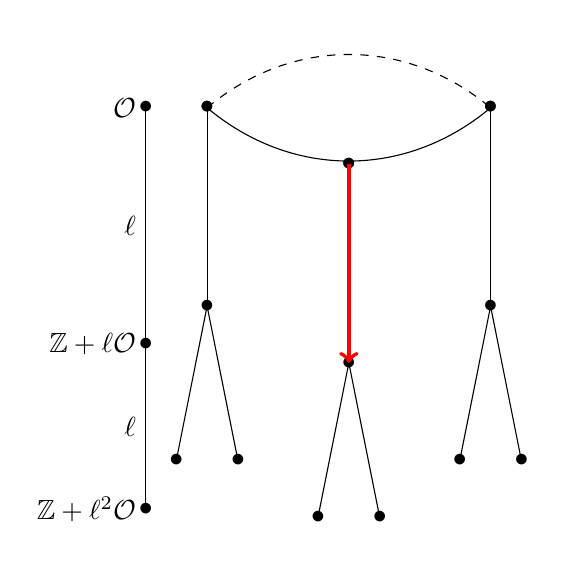
\begin{tikzpicture}[scale=0.60]
\coordinate (A) at (0,1.5);
\coordinate (AB) at (1,1.5);
%\coordinate (AZ) at (-1.5,1.5);	
\coordinate (B) at (0,5);
\coordinate (BB) at (1,5);
%\coordinate (BZ) at (-1.5,5.2);
%\coordinate (BZ2) at (-1.5,4.8);
\coordinate (C) at (0,10);
\coordinate (CB) at (1,10);
%\coordinate (CZ) at (-1.5,10);
\draw (A) node[left]{$\mathbb{Z} + \ell^2 \mathcal{O}$} node{$\bullet$};
\draw (B) node[left]{$\mathbb{Z} + \ell \mathcal{O}$} node{$\bullet$};
\draw (C) node[left]{$\mathcal{O}$} node{$\bullet$};
\draw (A)--(B)node[midway,left] {$\ell$};
\draw (B)--(C) node[midway,left] {$\ell$};
%\draw (CZ)--(BZ)[dashed]  node[midway,left] {$\ell$};
%\draw (BZ2)--(AZ)[dashed]  node[midway,left] {$\ell$};
\begin{scope}[yshift=10cm]
	\begin{scope}[xshift=4.3cm]
		\node (A) at (-3,0) {$\bullet$};
		\node (B) at (3,0) {$\bullet$};
		\node (C) at (270:1.2) {$\bullet$};
		\node (D) at (90:1.5) {};
		%\draw[-] (A.center) to[bend right=25] (C.center);
		\draw[-,dashed] (A.center) to[bend left=40] (B.center);
		%\draw[-] (B.center) to[bend left=25] (C.center);
		%\draw[-,dashed] (B.center) to[bend right] (D.center);
		\draw[-] (A.center) to[bend right=40] (B.center);
			\begin{scope}[xshift=-3cm]
			\coordinate (A) at (0,0);
			\coordinate (C) at (270:4.2);
			\coordinate (CA) at (265:7.5);
			\coordinate (CB) at (275:7.5);
			\draw (C)--(CA);
			\draw (C)--(CB);
			\draw (CA) node{$\bullet$};
			\draw (CB) node{$\bullet$};
			\draw (A) node{$\bullet$};
			\draw (C) node{$\bullet$};
			\draw (A)--(C);
			\end{scope}
			\begin{scope}[xshift=3cm]
			\coordinate (A) at (0,0);
			\coordinate (C) at (270:4.2);
			\coordinate (CA) at (265:7.5);
			\coordinate (CB) at (275:7.5);
			\draw (C)--(CA);
			\draw (C)--(CB);
			\draw (CA) node{$\bullet$};
			\draw (CB) node{$\bullet$};
			\draw (A) node{$\bullet$};
			\draw (C) node{$\bullet$};
			\draw (A)--(C);
			\end{scope}
			\begin{scope}[yshift=-1.2cm]
			\coordinate (A) at (0,0);
			\coordinate (C) at (270:4.2);
			\coordinate (CA) at (265:7.5);
			\coordinate (CB) at (275:7.5);
			\draw (C)--(CA);
			\draw (C)--(CB);
			\draw (CA) node{$\bullet$};
			\draw (CB) node{$\bullet$};
			\draw (A) node{$\bullet$};
			\draw (C) node{$\bullet$};
			\draw[line width=1.5pt,red,->] (A)--(C);
			\end{scope}
	\end{scope}
\end{scope}

%faire des fleches courbees avec les indices \ell et \ell^2


\end{tikzpicture}
\end{center}		
\end{figure}}

\only<2-2>{
\begin{figure}
\begin{center}

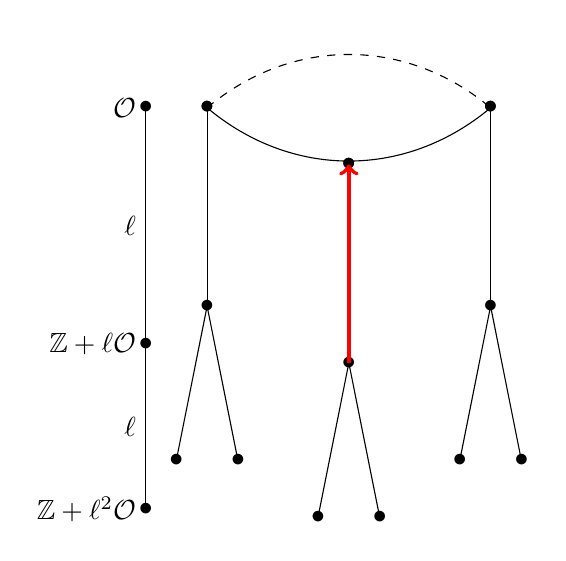
\begin{tikzpicture}[scale=0.60]
\coordinate (A) at (0,1.5);
\coordinate (AB) at (1,1.5);
%\coordinate (AZ) at (-1.5,1.5);	
\coordinate (B) at (0,5);
\coordinate (BB) at (1,5);
%\coordinate (BZ) at (-1.5,5.2);
%\coordinate (BZ2) at (-1.5,4.8);
\coordinate (C) at (0,10);
\coordinate (CB) at (1,10);
%\coordinate (CZ) at (-1.5,10);
\draw (A) node[left]{$\mathbb{Z} + \ell^2 \mathcal{O}$} node{$\bullet$};
\draw (B) node[left]{$\mathbb{Z} + \ell \mathcal{O}$} node{$\bullet$};
\draw (C) node[left]{$\mathcal{O}$} node{$\bullet$};
\draw (A)--(B)node[midway,left] {$\ell$};
\draw (B)--(C) node[midway,left] {$\ell$};
%\draw (CZ)--(BZ)[dashed]  node[midway,left] {$\ell$};
%\draw (BZ2)--(AZ)[dashed]  node[midway,left] {$\ell$};
\begin{scope}[yshift=10cm]
	\begin{scope}[xshift=4.3cm]
		\node (A) at (-3,0) {$\bullet$};
		\node (B) at (3,0) {$\bullet$};
		\node (C) at (270:1.2) {$\bullet$};
		\node (D) at (90:1.5) {};
		%\draw[-] (A.center) to[bend right=25] (C.center);
		\draw[-,dashed] (A.center) to[bend left=40] (B.center);
		%\draw[-] (B.center) to[bend left=25] (C.center);
		%\draw[-,dashed] (B.center) to[bend right] (D.center);
		\draw[-] (A.center) to[bend right=40] (B.center);
			\begin{scope}[xshift=-3cm]
			\coordinate (A) at (0,0);
			\coordinate (C) at (270:4.2);
			\coordinate (CA) at (265:7.5);
			\coordinate (CB) at (275:7.5);
			\draw (C)--(CA);
			\draw (C)--(CB);
			\draw (CA) node{$\bullet$};
			\draw (CB) node{$\bullet$};
			\draw (A) node{$\bullet$};
			\draw (C) node{$\bullet$};
			\draw (A)--(C);
			\end{scope}
			\begin{scope}[xshift=3cm]
			\coordinate (A) at (0,0);
			\coordinate (C) at (270:4.2);
			\coordinate (CA) at (265:7.5);
			\coordinate (CB) at (275:7.5);
			\draw (C)--(CA);
			\draw (C)--(CB);
			\draw (CA) node{$\bullet$};
			\draw (CB) node{$\bullet$};
			\draw (A) node{$\bullet$};
			\draw (C) node{$\bullet$};
			\draw (A)--(C);
			\end{scope}
			\begin{scope}[yshift=-1.2cm]
			\coordinate (A) at (0,0);
			\coordinate (C) at (270:4.2);
			\coordinate (CA) at (265:7.5);
			\coordinate (CB) at (275:7.5);
			\draw (C)--(CA);
			\draw (C)--(CB);
			\draw (CA) node{$\bullet$};
			\draw (CB) node{$\bullet$};
			\draw (A) node{$\bullet$};
			\draw (C) node{$\bullet$};
			\draw[line width=1.5pt,red,<-] (A)--(C);
			\end{scope}
	\end{scope}
\end{scope}

%faire des fleches courbees avec les indices \ell et \ell^2


\end{tikzpicture}
\end{center}		
\end{figure}}

\only<3-3>{
\begin{figure}
\begin{center}

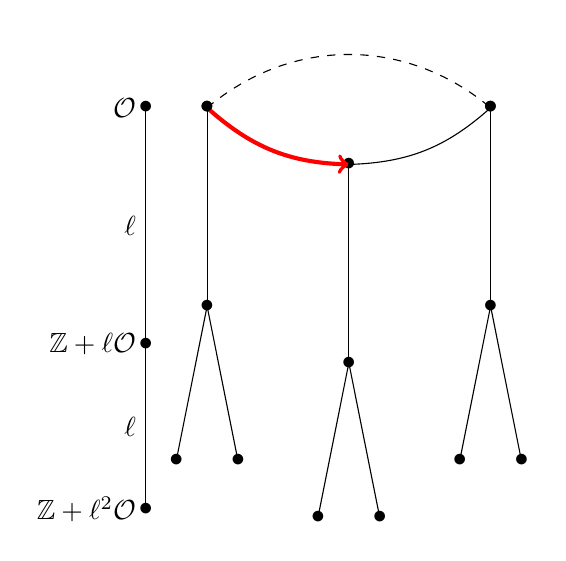
\begin{tikzpicture}[scale=0.60]
\coordinate (A) at (0,1.5);
\coordinate (AB) at (1,1.5);
%\coordinate (AZ) at (-1.5,1.5);	
\coordinate (B) at (0,5);
\coordinate (BB) at (1,5);
%\coordinate (BZ) at (-1.5,5.2);
%\coordinate (BZ2) at (-1.5,4.8);
\coordinate (C) at (0,10);
\coordinate (CB) at (1,10);
%\coordinate (CZ) at (-1.5,10);
\draw (A) node[left]{$\mathbb{Z} + \ell^2 \mathcal{O}$} node{$\bullet$};
\draw (B) node[left]{$\mathbb{Z} + \ell \mathcal{O}$} node{$\bullet$};
\draw (C) node[left]{$\mathcal{O}$} node{$\bullet$};
\draw (A)--(B)node[midway,left] {$\ell$};
\draw (B)--(C) node[midway,left] {$\ell$};
%\draw (CZ)--(BZ)[dashed]  node[midway,left] {$\ell$};
%\draw (BZ2)--(AZ)[dashed]  node[midway,left] {$\ell$};
\begin{scope}[yshift=10cm]
	\begin{scope}[xshift=4.3cm]
		\node (A) at (-3,0) {$\bullet$};
		\node (B) at (3,0) {$\bullet$};
		\node (C) at (270:1.2) {$\bullet$};
		\node (D) at (90:1.5) {};
		%\draw[-] (A.center) to[bend right=25] (C.center);
		\draw[-,dashed] (A.center) to[bend left=40] (B.center);
		%\draw[-] (B.center) to[bend left=25] (C.center);
		%\draw[-,dashed] (B.center) to[bend right] (D.center);
		\draw[-] (C.center) to[bend right=20] (B.center);
		\draw[line width=1.5pt,red,->] (A.center) to[bend right=20] (C.center);
			\begin{scope}[xshift=-3cm]
			\coordinate (A) at (0,0);
			\coordinate (C) at (270:4.2);
			\coordinate (CA) at (265:7.5);
			\coordinate (CB) at (275:7.5);
			\draw (C)--(CA);
			\draw (C)--(CB);
			\draw (CA) node{$\bullet$};
			\draw (CB) node{$\bullet$};
			\draw (A) node{$\bullet$};
			\draw (C) node{$\bullet$};
			\draw (A)--(C);
			\end{scope}
			\begin{scope}[xshift=3cm]
			\coordinate (A) at (0,0);
			\coordinate (C) at (270:4.2);
			\coordinate (CA) at (265:7.5);
			\coordinate (CB) at (275:7.5);
			\draw (C)--(CA);
			\draw (C)--(CB);
			\draw (CA) node{$\bullet$};
			\draw (CB) node{$\bullet$};
			\draw (A) node{$\bullet$};
			\draw (C) node{$\bullet$};
			\draw (A)--(C);
			\end{scope}
			\begin{scope}[yshift=-1.2cm]
			\coordinate (A) at (0,0);
			\coordinate (C) at (270:4.2);
			\coordinate (CA) at (265:7.5);
			\coordinate (CB) at (275:7.5);
			\draw (C)--(CA);
			\draw (C)--(CB);
			\draw (CA) node{$\bullet$};
			\draw (CB) node{$\bullet$};
			%\draw (A) node{$\bullet$};
			\draw (C) node{$\bullet$};
			\draw (A)--(C);
			\end{scope}
	\end{scope}
\end{scope}

%faire des fleches courbees avec les indices \ell et \ell^2


\end{tikzpicture}
\end{center}		
\end{figure}}


\end{column}
\begin{column}{4cm}
\begin{lem}[Kohel 1996]
$E$ and $E'$ two elliptic curves defined over $\mathbb{F}_q$, $\psi :E \rightarrow E'$ an $\ell$-isogeny. Then we say that $\psi$ is
\begin{enumerate}
\item  \textbf<1>{descending} if $\ell=[\mathcal{O} : \mathcal{O}']$
\pause
\item \textbf<2>{ascending} if $\ell=[\mathcal{O}':\mathcal{O}]$,
\pause 
\item \textbf<3>{horizontal} if $\mathcal{O}=\mathcal{O}'$.
\end{enumerate}
\end{lem}
%\begin{defi}
%The index $f=[\mathcal{O}_K : \mathcal{O}]$ is called the conductor of $\mathcal{O}$.
%\end{defi}
\end{column}

\end{columns}
\end{frame}

%%%%%%%%%%%%%%%%%%%%%%%%%%%%%%%%%%%%%%%%%%%%%%%%%%%%%%%%%%%%

\begin{frame}
    \begin{columns}
        \begin{column}{0.8\textwidth}
            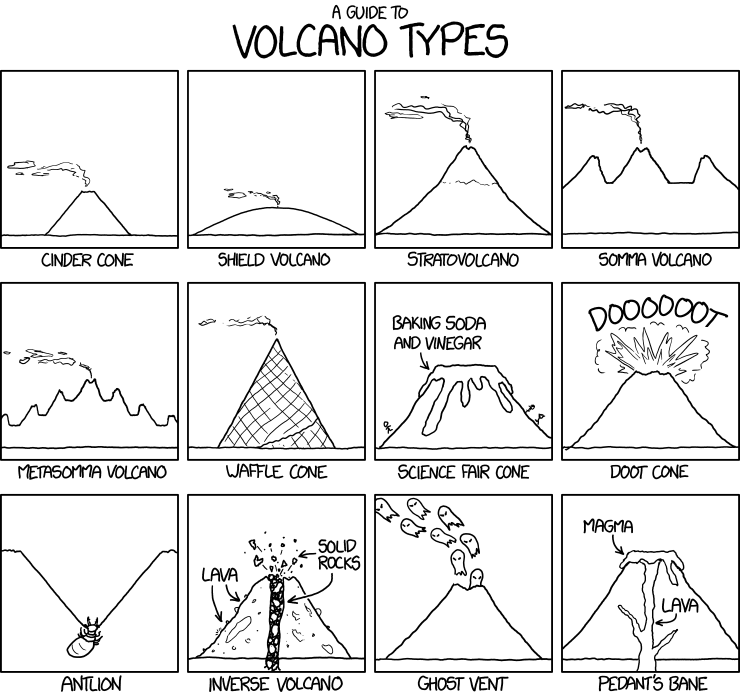
\includegraphics[height=\textheight]{Images/xkcd.png}
        \end{column}
        \begin{column}{0.2\textwidth}
            \href{http://xkcd.com/1714/}{xkcd.com/1714}
        \end{column}
    \end{columns}
\end{frame}

%%%%%%%%%%%%%%%%%%%%%%%%%%%%%%%%%%%%%%%%%%%%%%%%%%%%%%%%%%%%

\begin{frame}
\frametitle{The \textbf{real} guide to volcano types}
\begin{figure}[h]
		\begin{center}
        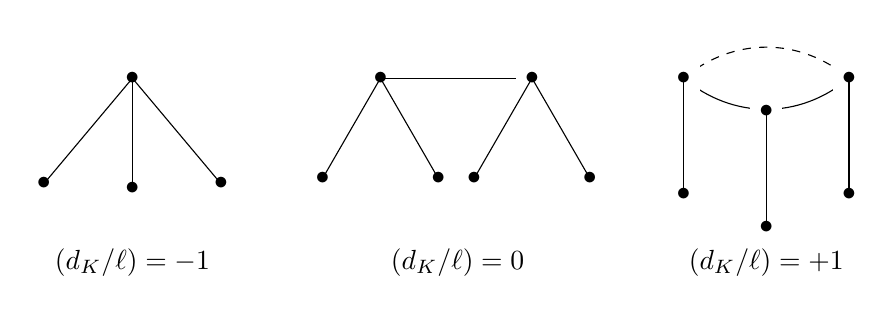
\begin{tikzpicture}[scale=0.35]
        \coordinate (A) at (0,0);
		\coordinate (B) at (230:5);
		\coordinate (C) at (270:4);
		\coordinate (D) at (310:5);
		\draw (A) node{$\bullet$};
		\draw (B) node[fill=white]{$\bullet$};
		\draw (C) node[fill=white]{$\bullet$};
		\draw (D) node[fill=white]{$\bullet$};
		\node at (0,-6.7) {$(d_K/\ell) = -1$};
		\draw (A)--(B);
		\draw (A)--(C);
		\draw (A)--(D);		
		\begin{scope}[xshift=9cm]
		\coordinate (A) at (0,0);
		\coordinate (B) at (5.5,0);
		\coordinate (C) at (240:4.2);
		\coordinate (D) at (300:4.2);
		\draw (A) node[fill=white]{$\bullet$};
		\draw (B) node[fill=white]{$\bullet$};
		\draw (C) node[fill=white]{$\bullet$};
		\draw (D) node[fill=white]{$\bullet$};
		\node at (2.8,-6.7) {$(d_K/\ell) = 0$};
		\draw (A)--(B);
		\draw (A)--(C);
		\draw (A)--(D);
		\end{scope}
		
		\begin{scope}[xshift=14.5cm]
		\coordinate (A) at (0,0);
		\coordinate (C) at (240:4.2);
		\coordinate (D) at (300:4.2);
		\draw (A) node[fill=white]{$\bullet$};
		\draw (C) node[fill=white]{$\bullet$};
		\draw (D) node[fill=white]{$\bullet$};
		\draw (A)--(C);
		\draw (A)--(D);
		\end{scope}
		
		\begin{scope}[xshift=23cm]
		\node (A) at (-3,0) {$\bullet$};
		\node (B) at (3,0) {$\bullet$};
		\node (C) at (270:1.2) {$\bullet$};
		\node (D) at (90:1.5) {};
		\node at (0,-6.7) {$(d_K/\ell) = +1$};
		%\draw[-] (A.center) to[bend right=25] (C.center);
		\draw[-,dashed] (A.center) to[bend left=40] (B.center);
		%\draw[-] (B.center) to[bend left=25] (C.center);
		%\draw[-,dashed] (B.center) to[bend right] (D.center);
		\draw[-] (A.center) to[bend right=40] (B.center);
			\begin{scope}[xshift=-3cm]
			\coordinate (A) at (0,0);
			\coordinate (C) at (270:4.2);
			\draw (A) node[fill=white]{$\bullet$};
			\draw (C) node[fill=white]{$\bullet$};
			\draw (A)--(C);
			\end{scope}
			\begin{scope}[xshift=3cm]
			\coordinate (A) at (0,0);
			\coordinate (C) at (270:4.2);
			\draw (A) node[fill=white]{$\bullet$};
			\draw (C) node[fill=white]{$\bullet$};
			\draw (A)--(C);
			\end{scope}
			\begin{scope}[yshift=-1.2cm]
			\coordinate (A) at (0,0);
			\coordinate (C) at (270:4.2);
			\draw (A) node[fill=white]{$\bullet$};
			\draw (C) node[fill=white]{$\bullet$};
			\draw (A)--(C);
			\end{scope}
		\end{scope}
		\end{tikzpicture}
		%\end{center}
		\caption{The three shapes of volcanoes of $2$-isogenies }
		
		\end{center} 
		\end{figure}
In the rest of this talk we consider only volcanoes with cyclic crater (Elikes' case).
%\begin{figure}[hbtp]
%\centering
%\includegraphics[scale=0.4]{Images/duo-volcan-wo-label.png}
%\caption{Volcano with one point on the crater, and two points}
%\end{figure}
\end{frame}

%%%%%%%%%%%%%%%%%%%%%%%%%%%%%%%%%%%%%%%%%%%%%%%%%%%%%%%%%%%%
%%%%%%%%%%%%%%%%%%%%%%%%%%%%%%%%%%%%%%%%%%%%%%%%%%%%%%%%%%%%

\section{An $\ell$-adic Couveignes' algorithm}

\begin{frame}
%Diapo sur le Frobenius....
%We want to study the action of the Frobenius on the $\ell$ torsion:
The Frobenius endomorphism acts on $E[\ell^k]$ as a $2\times2$ invertible matrix:
\[
\pi|E[\ell^k]:
\begin{pmatrix}
a & b \\
c & d 
\end{pmatrix} \bmod{\ell^k}
\]
\pause
It will be convenient to work with \emph{infinite} precision\dots

The projective limit of $E[\ell^k]$ as $k\to\infty$ is the \textit{Tate module} $T_\ell(E)$.

The Frobenius endomorphism acts on $T_\ell(E)$ as
\[
\pi|T_\ell(E) : \begin{pmatrix}
a & b \\
c & d  
\end{pmatrix} \in \mathrm{GL}_2(\mathbb{Z}_\ell).
\]

\begin{prop}
    In the Elkies case (cyclic crater)
    \[\pi^2 - t_\pi\pi + q = (\pi-{\color{red}\lambda})(\pi-{\color{blue}\mu})
    \qquad {\color{red}\lambda},{\color{blue}\mu}\in\mathbb{Z}_\ell.
    \]
    Hence $\pi|T_\ell(E)$ has two eigenvalues ${\color{red}\lambda},{\color{blue}\mu}$ over $\mathbb{Q}_\ell$.
\end{prop}
\end{frame}

%%%%%%%%%%%%%%%%%%%%%%%%%%%%%%%%%%%%%%%%%%%%%%%%%%%%%%%%%%%%

\begin{frame}

\begin{prop}\label{prop:matrice-Frobenius}
%Let $E$ be a curve on a crater of an $\ell$-isogeny volcano.
%Then there exists a unique $a \in \{ 0,\ell, \dots, \ell^{h-1}  \}$
%such that $\pi|T_\ell(E)$~is conjugate, over~$\mathbb{Z}_\ell$,
%to the matrix $\left ( \begin{smallmatrix}\lambda & a\\ 0 & \mu
%\end{smallmatrix}\right )$.
% where $a ∈ ℤ$, $0 ≤ a ≤ ℓ^{h} - 1$,
In the Elkies case the action of the Frobenius endomorphism $\pi$ on $T_\ell(E)$~is conjugate, over~$\mathbb{Z}_\ell$,
to a matrix \[\left ( \begin{matrix}{\color{red}\lambda} & a\\ 0 & {\color{blue}\mu} \end{matrix}\right ) \]  with $a \in \{ 0,1,\ell, \dots, \ell^{h-1}  \}$ and $a = 0$ if~$E$ lies on the crater.

%Moreover $a = 0$ if~$E$ lies on the crater.
%and else $h - v_{\ell}(a)$~is the depth of~$E$ in the volcano.
\end{prop}

\begin{figure}
\begin{center}

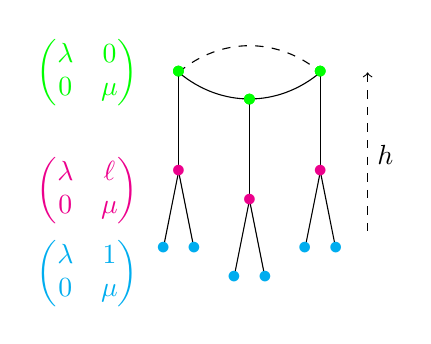
\begin{tikzpicture}[scale=0.30]
\coordinate (A) at (0,1.5);
\coordinate (AB) at (1,1.5);
\coordinate (AZ) at (-1.5,1.5);	
\coordinate (B) at (0,5);
\coordinate (BB) at (1,5);
\coordinate (BZ) at (-1.5,5.2);
\coordinate (BZ2) at (-1.5,4.8);
\coordinate (C) at (0,10);
\coordinate (CB) at (1,10);
\coordinate (CZ) at (-1.5,10);
\draw (A) node[left]{$\color{cyan}\left( \begin{matrix}
\lambda & 1 \\
0 & \mu
\end{matrix} \right) \color{black} $}; %node{$\bullet$};
\draw (B) node[left]{$\color{magenta} \left( \begin{matrix}
\lambda & \ell \\
0 & \mu
\end{matrix} \right) \color{black} $}; %node{$\bullet$};
\draw (C) node[left]{$\color{green} \left( \begin{matrix}
\lambda & 0 \\
0 & \mu
\end{matrix} \right) \color{black} $}; %node{$\bullet$};
%\draw (A)--(B);
%\draw (B)--(C);
%\draw (CZ)--(BZ)[dashed]  node[midway,left] {$\ell$};
%\draw (BZ2)--(AZ)[dashed]  node[midway,left] {$\ell$};
\begin{scope}[yshift=10cm]
	\begin{scope}[xshift=4.3cm]
		\node (A) at (-3,0) {$ \color{green} \bullet $};
		\node (B) at (3,0) {$  \color{green} \bullet$};
		\node (C) at (270:1.2) {$\color{green} \bullet \color{black}$};
		\node (D) at (90:1.5) {};
		%\draw[-] (A.center) to[bend right=25] (C.center);
		\draw[-,dashed] (A.center) to[bend left=40] (B.center);
		%\draw[-] (B.center) to[bend left=25] (C.center);
		%\draw[-,dashed] (B.center) to[bend right] (D.center);
		\draw[-] (A.center) to[bend right=40] (B.center);
		\draw (A) node{$ \color{green} \bullet $};
		\draw (B) node{$ \color{green} \bullet $};
		\draw (C) node{$ \color{green} \bullet $};
		%\draw[line width=2.5pt,red,->] (A.center) to[bend right=20] (C.center);
			\begin{scope}[xshift=-3cm]
			\coordinate (A) at (0,0);
			\coordinate (C) at (270:4.2);
			\coordinate (CA) at (265:7.5);
			\coordinate (CB) at (275:7.5);
			\draw (C)--(CA);
			\draw (C)--(CB);
			\draw (A)--(C);
			\draw (CA) node{$\color{cyan} \bullet$};
			\draw (CB) node{$\color{cyan} \bullet$};
			\draw (A) node{$ \color{green} \bullet \color{black}$};
			\draw (C) node{$ \color{magenta} \bullet \color{black}$};
			\end{scope}
			\begin{scope}[xshift=3cm]
			\coordinate (A) at (0,0);
			\coordinate (C) at (270:4.2);
			\coordinate (CA) at (265:7.5);
			\coordinate (CB) at (275:7.5);
			\draw (C)--(CA);
			\draw (C)--(CB);
			\draw (A)--(C);
			\draw (CA) node{$\color{cyan} \bullet$};
			\draw (CB) node{$\color{cyan}\bullet$};
			\draw (A) node{$\color{green} \bullet$};
			\draw (C) node{$\color{magenta} \bullet$};
			\end{scope}
			\begin{scope}[yshift=-1.2cm]
			\coordinate (A) at (0,0);
			\coordinate (C) at (270:4.2);
			\coordinate (CA) at (265:7.5);
			\coordinate (CB) at (275:7.5);
			\draw (C)--(CA);
			\draw (C)--(CB);
			\draw (A)--(C);
			\draw (CA) node{$\color{cyan} \bullet$};
			\draw (CB) node{$\color{cyan} \bullet$};
			%\draw (A) node{$\bullet$};
			\draw (C) node{$\color{magenta} \bullet$};
			\draw (A) node{$\color{green} \bullet$};
			
			
			%(C) node[left]{$\mathcal{O}$} node{$\bullet$};			
			
			\end{scope}
			\coordinate (F) at (5,0);
			\coordinate (G) at (5,-7);
			\draw[dashed,<-] (F)--(G) node[midway,right]{$h$};
	\end{scope}
\end{scope}

%faire des fleches courbees avec les indices \ell et \ell^2

\end{tikzpicture}
\end{center}
\end{figure}
\end{frame}

%%%%%%%%%%%%%%%%%%%%%%%%%%%%%%%%%%%%%%%%%%%%%%%%%%%%%%%%%%%%

\begin{frame}

\orangebox{In particular}{
If $E$ is on the crater, then $\pi|T_\ell(E)$ is conjugate over $\mathbb{Z}_\ell$ to
\[\left(
\begin{matrix}
{\color{red}\lambda} & 0 \\
0 & \color{blue}{\mu}
\end{matrix}
\right)\]
inducing a decomposition into eigenspaces
${\color{red}T_{\lambda}(E)} \oplus {\color{blue} T_{\mu}(E)}.$
}

\begin{itemize}
\item We shall restrict to the case where $E$ is on the crater.
\item We can reduce to this case using, e.g., [Fouquet Morain '01],
    [Miret, Moreno, Sadornil, Tena, Valls '06], [Ionica Joux '10].
\end{itemize}

\bluebox{Towards an $\ell$-adic Couveignes' algorithm}{
\begin{algorithmic}[1]
\REQUIRE $E, E'$ two $r$-isogenous curves on $\mathbb{F}_{q}$ 
\ENSURE $\phi: E \rightarrow E'$ of degree $r$
\end{algorithmic}}

\bluebox{}{\textbf{Fact:} $\phi$ maps ${\color{red}T_{\lambda}(E)\mapsto T_\lambda(E')}$ and 
${\color{blue} T_{\mu}(E) \mapsto T_\mu(E')}$.
}
\end{frame}

%%%%%%%%%%%%%%%%%%%%%%%%%%%%%%%%%%%%%%%%%%%%%%%%%%%%%%%%%%%%

\begin{frame}

\bluebox{Towards an $\ell$-adic Couveignes' algorithm}{
\begin{algorithmic}[1]
\REQUIRE $E, E'$ two $r$-isogenous curves on $\mathbb{F}_{q}$ 
\ENSURE $\phi: E \rightarrow E'$ of degree $r$
\end{algorithmic}}

\bluebox{}{\textbf{Fact:} $\phi$ maps ${\color{red}T_{\lambda}(E)\mapsto T_\lambda(E')}$ and 
${\color{blue} T_{\mu}(E) \mapsto T_\mu(E')}$.
 }

\begin{enumerate}
\item Fix $k$ such that  $\ell^{2k}>4r$
\item \textbf<3>{Compute bases of $T_\ell(E)$ and $T_\ell(E')$;}
\item Diagonalize $\to$ ${\color{red}T_\lambda(E)}\oplus\color{blue}T_\mu(E)$ and ${\color{red}T_\lambda(E')}\oplus\color{blue}T_\mu(E')$
\item Reduce $\to$ $\langle{\color{red}P},{\color{blue}Q}\rangle=E[\ell^k]$ and $\langle{\color{red}P'},{\color{blue}Q'}\rangle=E'[\ell^k]$;
\item For each \textbf{invertible diagonal} matrix
  $\left ( \begin{smallmatrix}a & 0\\ 0 & b
\end{smallmatrix}\right )$ in $(\mathbb{Z}/\ell^k \mathbb{Z})^{2 \times 2}$:
\hfill\only<2>{$O(r)$}
  \begin{enumerate}
  \item Compute the interpolation polynomial
    $L_{a,b}$ sending\\
    $\color{red}P\mapsto aP'$ and $\color{blue}Q\mapsto bQ'$;
  \item If $L_{a,b}$ defines an isogeny of degree $r$, return it and
    stop.
  \end{enumerate}
\end{enumerate}

\pause\pause

\orangebox{}{
\begin{center}
    Up to what precision do we need to compute $T_\ell(E)$ and $T_\ell(E')$?
\end{center}}
\end{frame}

%%%%%%%%%%%%%%%%%%%%%%%%%%%%%%%%%%%%%%%%%%%%%%%%%%%%%%%%%%%%


%\begin{frame}
%
%\begin{prop} \label{prop:diagonal-horizontal}
%Let~$E$ be a curve lying on the crater and~$P$ be a point of~$E[\ell^k]$.
%Then $ P$~is horizontal if and only if its preimages by multiplication by 
%$\ell^h$ are eigenvectors for~$\pi$.
%Let $P_0$ be such a preimage if $\pi(P_0) = \lambda P_0$ then we say that $P$~has direction~$\lambda$.
%\end{prop}
%
%Thus we will work only with curves for which we have $\pi|T_\ell(E)$ conjugate, over~$\mathbb{Z}_\ell$ to a diagonal matrix.
%
%\end{frame}


%\begin{frame}
%
%
%%Then the point $P=(36,96)$ computed as described earlier verifies that $\pi(P)=\lambda P$. Since $P$ is of order $2^3$ then we have $2^{2}P=(42,0)$ which is horizontal, the $2$-isogeny generated by $2^{2}P$ goes to another curve on the crater: $E2$. The points $2P$ is not necessarily horizontal. 
%\end{exe}
%\end{frame}

\begin{frame}
\frametitle{Computing $\red{T_{\lambda}(E)} \oplus \blu{T_{\mu}(E)} \bmod \ell^k $}
\begin{columns}
\begin{column}{6cm}
\begin{exe}[Volcano of height=0]

The ideals $\red{(\lambda,\ell)}$ and $\blu{(\mu,\ell)}$ of the class group $\mathrm{Cl}(K)$ act on the crater:

\begin{enumerate}
\item $\red{T_\lambda(E)\bmod\ell}$ and $\blu{T_\mu(E)\bmod\ell}$ are
    kernels of \textbf{horizontal isogenies} of opposite direction.
\item The directions are independent of the curve.
\end{enumerate}

In practice, 
\begin{itemize}
\item We compute $\red{P}\in E[\ell^k]$ such that $\pi(\color{red} {P} \color{black})= \color{red} \lambda {P}$;
\item Then $\red{\langle P\rangle = T_\lambda(E)  \bmod \ell^k}$.
\item Same for $\blu{T_\mu(E)}$.
\end{itemize}

\end{exe}

\end{column}
\begin{column}{6cm}
\begin{figure}[h]
	\begin{center}
	\begin{tikzpicture}[scale=0.4]
	\coordinate (A) at (0:5);
	\coordinate (B) at (45:5);
	\coordinate (C) at (90:5);
	\coordinate (D) at (135:5);
	\coordinate (E) at (180:5);
	\coordinate (F) at (225:5);
	\coordinate (G) at (270:5);
	\coordinate (H) at (315:5);
	\draw (A)--(B)--(C)--(D)--(E)--(F)--(G)--(H)--(A);		
	\draw[line width=1.5pt,red] (A)--(B) node[midway,right]{$\color{red} \lambda$};
	\draw[line width=1.5pt,blue] (A)--(H) node[midway,right]{$\color{blue} \mu$};
	\only<2->{
	    \draw[line width=1.5pt,red] (B)--(C) node[midway,above]{$\color{red} \lambda$};
	    \draw[line width=1.5pt,blue] (H)--(G) node[midway,below]{$\color{blue} \mu$};
	}
	\only<3>{
		\draw[line width=1.5pt,red] (C)--(D) node[midway,above]{$\color{red} \lambda$};
    	\draw[line width=1.5pt,blue] (G)--(F) node[midway,below]{$\color{blue} \mu$};
    }
    
	\draw (A) node{$\bullet$};
	\draw (A) node[right]{$E$};
	\draw (B) node{$\bullet$};
	\draw (C) node{$\bullet$};
	\draw (D) node{$\bullet$};
	\draw (E) node{$\bullet$};
	\draw (F) node{$\bullet$};
	\draw (G) node{$\bullet$};
	\draw (H) node{$\bullet$};
	\end{tikzpicture}	
	\end{center}
	\caption{
	    Isogenies generated by
	    \red{$\left( \lambda , \only<1>{\ell}\only<2>{\ell^2}\only<3>{\ell^3} \right)$},
	    \blu{$\left( \mu , \ell^{\only<2>{2}\only<3>{3}} \right)$}
	}
\end{figure}
\end{column}
\end{columns}
\end{frame}

%%%%%%%%%%%%%%%%%%%%%%%%%%%%%%%%%%%%%%%%%%%%%%%%%%%%%%%%%%%%

\begin{frame}
\only<2-2>{
\transdissolve
}
Assume we have \emph{diagonalized} $\pi$, i.e.\ we have $\langle\red P,\blu Q\rangle = E[\ell^k]$ s.t.
\[\pi:
\begin{pmatrix}\red P\\\blu Q\end{pmatrix} \mapsto
\begin{pmatrix}\red\lambda&0\\0&\blu\mu\end{pmatrix}
\begin{pmatrix}\red P\\\blu Q\end{pmatrix}
\]
\begin{itemize}
    \item If $h=0$, then $\red{\langle P\rangle = T_\lambda(E)}\bmod \ell^k$, $\blu{\langle Q\rangle =T_\mu(E)} \bmod \ell^k$;
    \hfill{\Large\Smiley}
    \item In general $\red{\langle P\rangle = T_\lambda(E)} \bmod \ell^{k-h}$, $\blu{\langle Q\rangle = T_\mu(E)} \bmod \ell^{k- h }$.
    \hfill{\Large\Sadey}
\end{itemize}

\begin{columns}
\begin{column}{5cm}
\orangebox{Volcano with height $h=0$}{
\begin{figure}[h]
	\begin{center}
	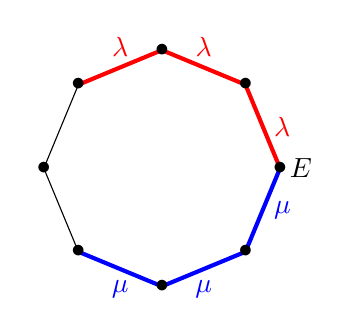
\begin{tikzpicture}[scale=0.3]
	\coordinate (A) at (0:5);
	\coordinate (B) at (45:5);
	\coordinate (C) at (90:5);
	\coordinate (D) at (135:5);
	\coordinate (E) at (180:5);
	\coordinate (F) at (225:5);
	\coordinate (G) at (270:5);
	\coordinate (H) at (315:5);
	\draw (A)--(B)--(C)--(D)--(E)--(F)--(G)--(H)--(A);		
	\draw[line width=1.5pt,red] (A)--(B) node[midway,right]{$\color{red} \lambda$};
	\draw[line width=1.5pt,blue] (A)--(H) node[midway,right]{$\color{blue} \mu$};
	\draw[line width=1.5pt,red] (B)--(C) node[midway,above]{$\color{red} \lambda$};
	\draw[line width=1.5pt,blue] (H)--(G) node[midway,below]{$\color{blue} \mu$};
	\draw[line width=1.5pt,red] (C)--(D) node[midway,above]{$\color{red} \lambda$};
	\draw[line width=1.5pt,blue] (G)--(F) node[midway,below]{$\color{blue} \mu$};
		
	\draw (A) node[right]{$E$};
	\draw (A) node{$\bullet$};
	\draw (B) node{$\bullet$};
	\draw (C) node{$\bullet$};
	\draw (D) node{$\bullet$};
	\draw (E) node{$\bullet$};
	\draw (F) node{$\bullet$};
	\draw (G) node{$\bullet$};
	\draw (H) node{$\bullet$};
	\end{tikzpicture}	
	\end{center}
\end{figure}
}
\end{column}
\begin{column}{5cm}
\orangebox{Volcano with height $h=2$}{
\begin{figure}[h]
		\begin{center}
\begin{tikzpicture}[scale=0.40]
\begin{scope}[yshift=10cm]
	\begin{scope}[xshift=4.3cm]
		\node[fill=pacificcream] (A) at (-3,0) {$E_3$};;
		\node[fill=pacificcream] (B) at (3,0) {$E_1$};
		\node[fill=pacificcream] (C) at (270:1.2) {$E$};
		\node[fill=pacificcream] (D) at (125:1.2) {$E_2$};
		%\draw[-] (A.center) to[bend right=25] (C.center);			
			\begin{scope}[xshift=-3cm]
			\coordinate (A) at (0,0);
			\coordinate (C) at (270:4.2);
			\coordinate (CA) at (265:7.5);
			\coordinate (CB) at (275:7.5);
			\coordinate (A2) at (0.15,0);
			\coordinate (C2) at (271.95:4.5);
			\only<1>{
			\draw [line width=1.5pt,color=red!30,->] (C)--(CB);
			\draw (C)--(CA);
			}
			\only<2>{
			\draw (C)--(CB);
			\draw [line width=1.5pt,color=red!30,->] (C)--(CA);			
			}
			\draw [line width=1.5pt,color=red!30,->] (A)--(C);
%			\draw (A) node[fill=white]{$30$};
%			\draw (C) node[fill=white]{$98$};
%			\draw (CA) node[fill=white]{$22$};
%			\draw (CB) node[fill=white]{$74$};
%			\draw (A) node[fill=pacificcream]{$E_2$};
			\draw (C) node[fill=pacificcream]{$\bullet$};
			\draw (CA) node[fill=pacificcream]{$\bullet$};
			\draw (CB) node[fill=pacificcream]{$\bullet$};
			\end{scope}
			\begin{scope}[xshift=3cm]
			\coordinate (A) at (0,0);
			\coordinate (C) at (270:4.2);
			\coordinate (CA) at (265:7.5);
			\coordinate (CB) at (275:7.5);
			\only<1-1>{
			\draw [line width=1.5pt,color=blue!30,->] (C)--(CA);
			\draw [line width=1.5pt,color=blue!30,->] (A)--(C);}
			\only<2-2>{
			\draw (C)--(CA);
			\draw (A)--(C);			
			}
			\draw (C)--(CB);
%			\draw (A) node[fill=white]{$65$};
%			\draw (C) node[fill=white]{$60$};
%			\draw (CA) node[fill=white]{$39$};
%			\draw (CB) node[fill=white]{$62$};
%			\draw (A) node[fill=pacificcream]{$E_1$};
			\draw (C) node[fill=pacificcream]{$\bullet$};
			\draw (CA) node[fill=pacificcream]{$\bullet$};
			\draw (CB) node[fill=pacificcream]{$\bullet$};
			\end{scope}
			\begin{scope}[yshift=-1.2cm]
			\coordinate (A) at (0,0);
			\coordinate (C) at (270:4.2);
			\coordinate (CA) at (265:7.5);
			\coordinate (CB) at (275:7.5);
			\draw (C)--(CA);
			\draw (C)--(CB);
			\draw (A)--(C);
%			\draw (A) node[fill=white]{$28$};
%			\draw (C) node[fill=white]{$27$};
%			\draw (CA) node[fill=white]{$45$};
%			\draw (CB) node[fill=white]{$68$};
%			\draw (A) node[fill=pacificcream]{$E$};
			\draw (C) node[fill=pacificcream]{$\bullet$};
			\draw (CA) node[fill=pacificcream]{$\bullet$};
			\draw (CB) node[fill=pacificcream]{$\bullet$};
			\end{scope}
			\begin{scope}[shift={(D)}]
			\coordinate (A) at (0,0);
			\coordinate (C) at (270:4.2);
			\coordinate (CA) at (265:7.5);
			\coordinate (CB) at (275:7.5);
			\draw [dashed] (C)--(CA);
			\draw [dashed] (C)--(CB);
			\only<1>{\draw [dashed] (A)--(C);}
			\only<2>{\draw [dashed] (A)--(C);}
			\draw (C) node[fill=pacificcream,]{$\bullet$};
			\draw (CA) node[color=black!90]{$\bullet$};
			\draw (CB) node[color=black!90]{$\bullet$};
			\end{scope}
	\node[fill=pacificcream] (A) at (-3,0) {$E_3$};;
	\node[fill=pacificcream] (B) at (3,0) {$E_1$};
	\node[fill=pacificcream] (C) at (270:1.2) {$E$};
	\node[fill=pacificcream] (D) at (125:1.2) {$E_2$};
	\only<1>{
	\draw[-] (A.center) to[bend left=40] (B.center);
	}
	\only<2>{
	\draw[-,line width=1.5pt,color=blue] (D.center) to[bend left=30] (B.center);
	\draw[-,line width=1.5pt,color=blue] (D.center) to[bend right=30] (A.center);
	}
	%\draw[-] (B.center) to[bend left=25] (C.center);
	%\draw[-,dashed] (B.center) to[bend right] (D.center);
	\draw[line width=1.5pt,blue,->] (C.center) to[bend right=20] (B.center);
	\draw [line width=1.5pt,red,<-] (A.center) to[bend right=20] (C.center);		
	\node[fill=pacificcream] (A) at (-3,0) {$E_3$};;
	\node[fill=pacificcream] (B) at (3,0) {$E_1$};
	\node[fill=pacificcream] (C) at (270:1.2) {$E$};
	\node[fill=pacificcream] (D) at (125:1.2) {$E_2$};
	\end{scope}
\end{scope}
\end{tikzpicture}
		%\end{center}
		%\caption{Volcano of $2$-isogenies with height $h=2$}
		
		\end{center} 
		\end{figure}
}
\end{column}
\end{columns}
\end{frame}

%%%%%%%%%%%%%%%%%%%%%%%%%%%%%%%%%%%%%%%%%%%%%%%%%%%%%%%%%%%%

\begin{frame}
%Frame sur les bases horizontales, diagonales.
\begin{defi}[Horizontal and diagonal bases]
  Let~$E$ be a curve on the crater. We call a
  basis of~$E[\ell^k]$
\begin{itemize}
		  
 {\setlength\itemindent{25pt} \item[\emph{diagonal}] if $\pi$~acts as a diagonal matrix on it;}
  {\setlength\itemindent{25pt} \item[\emph{horizontal}] if both basis points generate kernels of
  horizontal $\ell^k$-isogenies. }

\end{itemize}  
\end{defi}

\orangebox{Facts}{
\begin{itemize}
\item Horizontal $\Rightarrow$ diagonal.
\item Diagonal $\Rightarrow$ horizontal iff $h=0$.
\item $\red{T_\lambda(E) \bmod\ell^k}$ and $\blu{T_\mu(E) \bmod\ell^k}$ form a horizontal basis.
\end{itemize}
}

\begin{center}
    \textbf{Our goal:} Given a diagonal basis $\to$ compute a horizontal one.
\end{center}
\end{frame}

%%%%%%%%%%%%%%%%%%%%%%%%%%%%%%%%%%%%%%%%%%%%%%%%%%%%%%%%%%%%

% \begin{frame}
% \begin{columns}

% \begin{column}{4cm}
% \begin{exe}[Volcano with height=2]
% Let $E_0$ be a curve on a cyclic crater of a volcano of $2$-isogenies.
% %with $j$-invariant $28$ and defined on $\mathbb{F}_{101}$ by: 
% %\[y^2=x^3+85x+11\]
% %$P=(36,96)$ a point of order $8$ verifies that $\pi(P)=\lambda P$

% Let $P$ be a point of order $8$ such that $\pi(P)=\color{red}\lambda \color{black}P$

% \begin{itemize}\only<1-1>{
% \item \boldmath $P$ \unboldmath is  \textbf{not horizontal},}
% \only<2-3>{\item $P$ is not horizontal,}
% \only<2-2>{\item \boldmath $2P$ \unboldmath is \textbf{not horizontal},}
% \only<1,3>{\item $2P$ is not horizontal,}
% \only<1-2>{\item $2^{2}P$ is horizontal.}
% \only<3-3>{\item \boldmath $2^2P$ \unboldmath is \textbf{horizontal}.}
% \end{itemize}


% \end{exe}
% \end{column}

% \begin{column}{7cm}
% \begin{figure}[h]
% 		\begin{center}
		
% \begin{tikzpicture}[scale=0.60]
% \begin{scope}[yshift=10cm]
% 	\begin{scope}[xshift=4.3cm]
% 		\node (A) at (-3,0) {$\bullet$};
% 		\node (B) at (3,0) {$\bullet$};
% 		\node (C) at (270:1.2) {$\bullet$};
% 		\node (D) at (90:1.5) {};
% 		%\draw[-] (A.center) to[bend right=25] (C.center);
% 		\draw[-] (A.center) to[bend left=40] (B.center);
% 		%\draw[-] (B.center) to[bend left=25] (C.center);
% 		%\draw[-,dashed] (B.center) to[bend right] (D.center);
% 		\draw[-] (C.center) to[bend right=20] (B.center);
% 		\draw [line width=1.5pt,red,<-] (A.center) to[bend right=20] (C.center);
% 			\begin{scope}[xshift=-3cm]
% 			\coordinate (A) at (0,0);
% 			\coordinate (C) at (270:4.2);
% 			\coordinate (CA) at (265:7.5);
% 			\coordinate (CB) at (275:7.5);
% 			\draw (C)--(CA);
% 			\only<1-1>{
% 			\draw [line width=1.5pt,color=red!30,->] (C)--(CB);
% 			}
% 			\only<2-3>{
% 			\draw (C)--(CB);
% 			}
% 			\only<1-2>{
% 			\draw [line width=1.5pt,color=red!30,->] (A)--(C);
% 			}
% 			\only<3-3>{
% 			\draw (A)--(C);			
% 			}
% %			\draw (A) node[fill=white]{$30$};
% %			\draw (C) node[fill=white]{$98$};
% %			\draw (CA) node[fill=white]{$22$};
% %			\draw (CB) node[fill=white]{$74$};
% 			\draw (A) node[fill=white]{$E_2$};
% 			\draw (C) node[fill=white]{$\bullet$};
% 			\draw (CA) node[fill=white]{$\bullet$};
% 			\draw (CB) node[fill=white]{$\bullet$};
% 			\end{scope}
% 			\begin{scope}[xshift=3cm]
% 			\coordinate (A) at (0,0);
% 			\coordinate (C) at (270:4.2);
% 			\coordinate (CA) at (265:7.5);
% 			\coordinate (CB) at (275:7.5);
% 			\draw (C)--(CA);
% 			\draw (C)--(CB);
% 			\draw (A)--(C);
% %			\draw (A) node[fill=white]{$65$};
% %			\draw (C) node[fill=white]{$60$};
% %			\draw (CA) node[fill=white]{$39$};
% %			\draw (CB) node[fill=white]{$62$};
% 			\draw (A) node[fill=white]{$E_1$};
% 			\draw (C) node[fill=white]{$\bullet$};
% 			\draw (CA) node[fill=white]{$\bullet$};
% 			\draw (CB) node[fill=white]{$\bullet$};
% 			\end{scope}
% 			\begin{scope}[yshift=-1.2cm]
% 			\coordinate (A) at (0,0);
% 			\coordinate (C) at (270:4.2);
% 			\coordinate (CA) at (265:7.5);
% 			\coordinate (CB) at (275:7.5);
% 			\draw (C)--(CA);
% 			\draw (C)--(CB);
% 			\draw (A)--(C);
% %			\draw (A) node[fill=white]{$28$};
% %			\draw (C) node[fill=white]{$27$};
% %			\draw (CA) node[fill=white]{$45$};
% %			\draw (CB) node[fill=white]{$68$};
% 			\draw (A) node[fill=white]{$E_0$};
% 			\draw (C) node[fill=white]{$\bullet$};
% 			\draw (CA) node[fill=white]{$\bullet$};
% 			\draw (CB) node[fill=white]{$\bullet$};
% 			\end{scope}
% 	\end{scope}
% \end{scope}
% \end{tikzpicture}
% 		%\end{center}
% 		\caption{Volcano of $2$-isogenies on $\mathbb{F}_{101}$}
		
% 		\end{center} 
% 		\end{figure}
% \end{column}
% \end{columns}
% \end{frame}

%%%%%%%%%%%%%%%%%%%%%%%%%%%%%%%%%%%%%%%%%%%%%%%%%%%%%%%%%%%%

\begin{frame}
\frametitle{How to \textit{straighten} a diagonal basis}
\begin{columns}

\begin{column}{4cm}
\begin{exe}[$h=2$]
We are given a diagonal basis $\langle\red P,\blu Q\rangle = E[\ell^k]$ 
\[
\begin{pmatrix}\red P\\\blu Q\end{pmatrix}
\mapsto
\left( \begin{matrix}
\red{\lambda} & 0 \\
0 & \blue \mu 
\end{matrix} \right) 
\begin{pmatrix}\red P\\\blu Q\end{pmatrix}
\]

Assume that $k \geqslant h+1$.
\end{exe}
\end{column}

\begin{column}{7cm}
\begin{figure}[h]
		\begin{center}
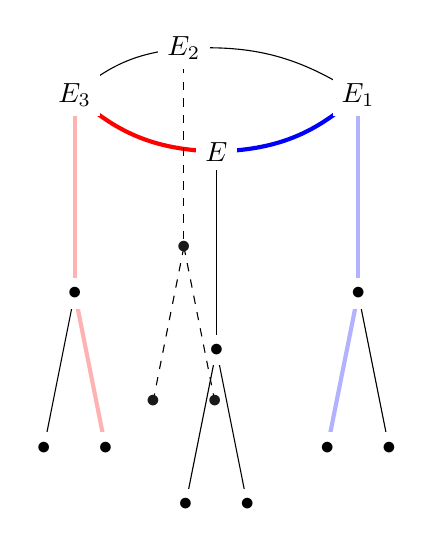
\begin{tikzpicture}[scale=0.60]
\begin{scope}[yshift=10cm]
	\begin{scope}[xshift=4.3cm]
		\node (A) at (-3,0) {$\bullet$};
		\node (B) at (3,0) {$\bullet$};
		\node (C) at (270:1.2) {$\bullet$};
		\node (D) at (125:1.2) {$E_2$};
		%\draw[-] (A.center) to[bend right=25] (C.center);
		\draw[-] (D.center) to[bend left=18] (B.center);
		\draw[-] (D.center) to[bend right=18] (A.center);
		%\draw[-] (B.center) to[bend left=25] (C.center);
		%\draw[-,dashed] (B.center) to[bend right] (D.center);
		\draw[line width=1.5pt,blue,->] (C.center) to[bend right=20] (B.center);
		\draw [line width=1.5pt,red,<-] (A.center) to[bend right=20] (C.center);
			\begin{scope}[xshift=-3cm]
			\coordinate (A) at (0,0);
			\coordinate (C) at (270:4.2);
			\coordinate (CA) at (265:7.5);
			\coordinate (CB) at (275:7.5);
			\draw (C)--(CA);
			\draw [line width=1.5pt,color=red!30,->] (C)--(CB);
			\draw [line width=1.5pt,color=red!30,->] (A)--(C);
%			\draw (A) node[fill=white]{$30$};
%			\draw (C) node[fill=white]{$98$};
%			\draw (CA) node[fill=white]{$22$};
%			\draw (CB) node[fill=white]{$74$};
			\draw (A) node[fill=white]{$E_3$};
			\draw (C) node[fill=white]{$\bullet$};
			\draw (CA) node[fill=white]{$\bullet$};
			\draw (CB) node[fill=white]{$\bullet$};
			\end{scope}
			\begin{scope}[xshift=3cm]
			\coordinate (A) at (0,0);
			\coordinate (C) at (270:4.2);
			\coordinate (CA) at (265:7.5);
			\coordinate (CB) at (275:7.5);
			\draw [line width=1.5pt,color=blue!30,->] (C)--(CA);
			\draw (C)--(CB);
			\draw [line width=1.5pt,color=blue!30,->] (A)--(C);
%			\draw (A) node[fill=white]{$65$};
%			\draw (C) node[fill=white]{$60$};
%			\draw (CA) node[fill=white]{$39$};
%			\draw (CB) node[fill=white]{$62$};
			\draw (A) node[fill=white]{$E_1$};
			\draw (C) node[fill=white]{$\bullet$};
			\draw (CA) node[fill=white]{$\bullet$};
			\draw (CB) node[fill=white]{$\bullet$};
			\end{scope}
			\begin{scope}[yshift=-1.2cm]
			\coordinate (A) at (0,0);
			\coordinate (C) at (270:4.2);
			\coordinate (CA) at (265:7.5);
			\coordinate (CB) at (275:7.5);
			\draw (C)--(CA);
			\draw (C)--(CB);
			\draw (A)--(C);
%			\draw (A) node[fill=white]{$28$};
%			\draw (C) node[fill=white]{$27$};
%			\draw (CA) node[fill=white]{$45$};
%			\draw (CB) node[fill=white]{$68$};
			\draw (A) node[fill=white]{$E$};
			\draw (C) node[fill=white]{$\bullet$};
			\draw (CA) node[fill=white]{$\bullet$};
			\draw (CB) node[fill=white]{$\bullet$};
			\end{scope}
			\begin{scope}[shift={(D)}]
			\coordinate (A) at (0,0);
			\coordinate (C) at (270:4.2);
			\coordinate (CA) at (265:7.5);
			\coordinate (CB) at (275:7.5);
			\draw [dashed] (C)--(CA);
			\draw [dashed] (C)--(CB);
			\draw [dashed] (A)--(C);
			\draw (A) node[fill=white]{$E_2$};
			\draw (C) node[color=black!90]{$\bullet$};
			\draw (CA) node[color=black!90]{$\bullet$};
			\draw (CB) node[color=black!90]{$\bullet$};
			\end{scope}
	\end{scope}
\end{scope}
\end{tikzpicture}

		\end{center} 
		\end{figure}
\end{column}
\end{columns}
\end{frame}

%%%%%%%%%%%%%%%%%%%%%%%%%%%%%%%%%%%%%%%%%%%%%%%%%%%%%%%%%%%%

\begin{frame}
\frametitle{How to \textit{straighten} a diagonal basis}
\only<2-2>{
\transdissolve
}
\only<4-4>{
\transdissolve
}

\begin{columns}
\begin{column}{6cm}
\orangebox{}{
\raggedright
$\red P \in E$ is diagonal, and $\ell$-horizontal:
\[\red{ \langle P \rangle = T_\lambda(E) \mod \ell}\]

$\blu\psi(\red P) \in E_1$ is also diagonal\uncover<2->{, and \mbox{$\ell^2$-horizontal}:
    \[\red{ \langle \blu\psi(\red P) \rangle = T_\lambda(E) \mod \ell^2}\]}
    
\vspace{-2mm}

\begin{itemize}
\item<3-> We continue until we have a horizontal point $\red{P_{k-1}}\in E_{k-1}$;
\item<4-> We apply the same procedure to get back to $E$.
\item<5-> We repeat again the procedure for $\blu Q\in E$.
\end{itemize}
}


\end{column}
\begin{column}{6cm}
\begin{figure}
\begin{center}
\begin{tikzpicture}[scale=0.60]
\begin{scope}[yshift=10cm]
	\begin{scope}[xshift=4.3cm]
		\node (A) at (-3,0) {$\bullet$};
		\node (B) at (3,0) {$\bullet$};
		\node (C) at (270:1.2) {$\bullet$};
		\node (D) at (125:1.2) {$E_2$};
		%\draw[-] (A.center) to[bend right=25] (C.center);
		\only<1-2>{		
		\draw[-] (D.center) to[bend left=18] (B.center);
		\draw[-] (D.center) to[bend right=20] (A.center);
		}
		\only<3-3>{
		\draw[line width=1.5pt,blue,->] (D.center) to[bend left=20] (B.center);
		\draw[-] (D.center) to[bend right=20] (A.center);
		\node (F) at (1.25,1.30) {$\color{blue} \mu$};
		\node (F2) at (1.25,0.50) {$\color{blue} \psi_2$};		
		}
		\only<4->{
		\draw[line width=1.5pt,red,->] (D.center) to[bend left=20] (B.center);
		\draw[-] (D.center) to[bend right=20] (A.center);
		\node (F) at (1.25,1.30) {$\color{red} \lambda$};		
		}
		%\draw[-] (B.center) to[bend left=25] (C.center);
		%\draw[-,dashed] (B.center) to[bend right] (D.center);
		\only<1-1>{
		\draw[line width=1.5pt,blue,->] (C.center) to[bend right=20] (B.center); 
		\node (F) at (1.5,-0.5) {$\color{blue} \mu$};	
		\node (F2) at (1.5,-1.5) {$\color{blue} \psi$};	
		}
		\only<2->{
		\draw[line width=1.5pt,red,<-] (C.center) to[bend right=20] (B.center); 
		\node (F) at (1.5,-0.5) {$\color{red} \lambda$};		
		}
		\draw [line width=1.5pt,red,<-] (A.center) to[bend right=20] (C.center);
		\node (E) at (-1.5,-0.5) {$\color{red} \lambda$};
		
			\begin{scope}[xshift=-3cm]
			\coordinate (A) at (0,0);
			\coordinate (C) at (270:4.2);
			\coordinate (CA) at (265:7.5);
			\coordinate (CB) at (275:7.5);
			\draw (C)--(CA);
			\only<1-1>{
			\draw [line width=1.5pt,color=red!30,->] (C)--(CB);}
			\only<2->{
			\draw (C)--(CB);}
			\only<1-3>{			
			\draw [line width=1.5pt,color=red!30,->] (A)--(C);}
			\only<4->{
			\draw (A)--(C);}
%			\draw (A) node[fill=white]{$30$};
%			\draw (C) node[fill=white]{$98$};
%			\draw (CA) node[fill=white]{$22$};
%			\draw (CB) node[fill=white]{$74$};
			\draw (A) node[fill=white]{$E_3$};
			\draw (C) node[fill=white]{$\bullet$};
			\draw (CA) node[fill=white]{$\bullet$};
			\draw (CB) node[fill=white]{$\bullet$};
			\end{scope}
			\begin{scope}[xshift=3cm]
			\coordinate (A) at (0,0);
			\coordinate (C) at (270:4.2);
			\coordinate (CA) at (265:7.5);
			\coordinate (CB) at (275:7.5);
			\draw (C)--(CA);
			\draw (C)--(CB);
			\draw (A)--(C);
%			\draw (A) node[fill=white]{$65$};
%			\draw (C) node[fill=white]{$60$};
%			\draw (CA) node[fill=white]{$39$};
%			\draw (CB) node[fill=white]{$62$};
			\draw (A) node[fill=white]{$E_1$};
			\only<2-3>{\draw (A) node[fill=yellow!50!white,shape=circle]{$E_1$};}
			\draw (C) node[fill=white]{$\bullet$};
			\draw (CA) node[fill=white]{$\bullet$};
			\draw (CB) node[fill=white]{$\bullet$};
			\end{scope}
			\begin{scope}[yshift=-1.2cm]
			\coordinate (A) at (0,0);
			\coordinate (C) at (270:4.2);
			\coordinate (CA) at (265:7.5);
			\coordinate (CB) at (275:7.5);
			\draw (C)--(CA);
			\draw (C)--(CB);
			\draw (A)--(C);
			\draw (A) node[fill=white]{$E$};
			\only<1>{\draw (A) node[fill=yellow!50!white,shape=circle]{$E$};}
			\draw (C) node[fill=white]{$\bullet$};
			\draw (CA) node[fill=white]{$\bullet$};
			\draw (CB) node[fill=white]{$\bullet$};
%			\draw (CA) node[fill=white]{$45$};
%			\draw (CB) node[fill=white]{$68$};
			\end{scope}
			\begin{scope}[shift={(D)}]
			\coordinate (A) at (0,0);
			\coordinate (C) at (270:4.2);
			\coordinate (CA) at (265:7.5);
			\coordinate (CB) at (275:7.5);
			\draw [dashed] (C)--(CA);
			\draw [dashed] (C)--(CB);
			\draw [dashed] (A)--(C);
			\draw (C) node[color=black!90]{$\bullet$};
			\draw (CA) node[color=black!90]{$\bullet$};
			\draw (CB) node[color=black!90]{$\bullet$};
			\only<1-3>{\draw (A) node[fill=white]{$E_2$};}			
			\only<4->{\draw (A) node[fill=yellow!50!white,shape=circle]{$E_2$};}
			\end{scope}
	\end{scope}
\end{scope}
\end{tikzpicture}
\end{center}
\end{figure}
\end{column}
\end{columns}
\end{frame}


%%%%%%%%%%%%%%%%%%%%%%%%%%%%%%%%%%%%%%%%%%%%%%%%%%%%%%%%%%%%


\begin{frame}
\frametitle{An $\ell$-adic Couveignes' algorithm}
\bluebox{$\ell$-adic Couveignes' algorithm (crater curves only)}{
\begin{enumerate}
\item Fix $k$ such that  $\ell^{2k}>4r$
\item Compute \textbf{horizontal} bases $(\color{red}P\color{black},\color{blue}Q\color{black})$ of
  $E[\ell^k]$ and $(\color{red}P'\color{black},\color{blue}Q'\color{black})$ of $E'[\ell^k]$;
\item Compute the polynomial~$T=\prod(X-x_i)$ of degree $\frac{\ell^{2k}-1}{2}$
  with $x_i$ x-coordinates of $\langle \color{red}P\color{black},\color{blue}Q\color{black}\rangle$; %using the method of
  %[De Feo '10] and [Enge-Morain '03];
\item For each \textbf{invertible diagonal} matrix
  $\left ( \begin{smallmatrix}a & 0\\ 0 & b
\end{smallmatrix}\right )$ in $(\mathbb{Z}/\ell^k \mathbb{Z})^{2 \times 2}$:
  \begin{enumerate}
  \item compute the interpolation polynomial
    $L_{a,b}$ such that
    $L_{a,b} (x (u \color{red}P\color{black} + v \color{blue}Q\color{black})) = x(a\, u\,\color{red}P'\color{black} + b\,v\, \color{blue}Q'\color{black})$ for all
    $u, v \in \mathbb{Z}/\ell^k \mathbb{Z}$;
  \item Use an algorithm of rational reconstruction 
    to compute a rational
    fraction $F_{a,b}=L_{a,b}\bmod{T}$ of degrees~$(r, r-1)$;
  \item If $F_{a,b}$ defines an isogeny of degree $r$, return it and
    stop.
  \end{enumerate}
\end{enumerate}}
\end{frame}


%%%%%%%%%%%%%%%%%%%%%%%%%%%%%%%%%%%%%%%%%%%%%%%%%%%%%%%%%%%%
%%%%%%%%%%%%%%%%%%%%%%%%%%%%%%%%%%%%%%%%%%%%%%%%%%%%%%%%%%%%

\section{Conclusion}

%\begin{frame}
%\frametitle{Improving interpolation with the Frobenius}
%\begin{figure}[h]
%\begin{center}
%
%\begin{tikzpicture}[scale=0.3]
%        \coordinate (A) at (0,0);
%        \coordinate (AB) at (-9,4.25);
%		\coordinate (AC) at (9,4.25);
%		\draw (A)--(AB);
%		\draw (A)--(AC);
%		\draw (A) node[fill=white]{$\color{red}{T_3}$};
%		
%
%		\coordinate (ABA) at (-12.63,8.5);
%		%\coordinate (ABA) at (-11.63,8.5);
%		
%		\draw (ABA)--(AB);
%		
%		\coordinate (ABAb) at (-15.26,12.75);
%		%\coordinate (ABAb) at (-14.26,12.75);
%		
%		\draw (ABA)--(ABAb);
%		\draw (ABAb) node[fill=white]{$\color{red}{T_0}$};
%		
%		\coordinate (ABAa) at (-10,12.75);
%		%\coordinate (ABAa) at (-9,12.75);
%		
%		
%		\draw (ABA)--(ABAa);
%		\draw (ABA) node[fill=white]{$\color{red}{T_1}$};
%		\draw (ABAa) node[fill=white][left]{$\color{red}{\pi^4(T_0)}$};%ancien \pi(T)
%		
%		\coordinate (ACA) at (-5.37,8.5);
%		%\coordinate (ACA) at (-6.37,8.5);
%		
%		
%		\draw (AB)--(ACA);
%		\draw (AB) node[fill=white]{$\color{red}{T_2}$};
%		\coordinate (ACAa) at (-8,12.75);
%		%\coordinate (ACAa) at (-9,12.75);
%		
%		
%		\draw (ACA)--(ACAa);
%		\draw (ACAa) node[fill=white]{$\pi^2(T_0)$};%ancien \pi^2(T)
%		
%		\coordinate (ACAb) at (-2.74,12.75);
%		%\coordinate (ACAb) at (-3.74,12.75);
%		
%		
%		\draw (ACA)--(ACAb);
%		\draw (ACAb) node[fill=white]{$\pi^6(T_0)$};%ancien \pi^3(T)
%		\draw (ACA) node[fill=white]{$\color{red}{\pi^2(T_1)}$};% ancien \pi^2(T_2)
%		
%		\begin{scope}[xshift=18cm]
%		\coordinate (ABA) at (-12.63,8.5);
%		%\coordinate (ABA) at (-11.63,8.5);
%
%		\draw (ABA)--(AC);
%		
%		\coordinate (ABAb) at (-15.26,12.75);
%		%\coordinate (ABAb) at (-14.26,12.75);
%		
%		\draw (ABA)--(ABAb);
%		\draw (ABAb) node[fill=white]{$\pi(T_0)$};%ancien \pi^4(T)
%		
%		\coordinate (ABAa) at (-9.7,12.75);
%		%\coordinate (ABAa) at (-9,12.75);
%		
%		
%		\draw (ABA)--(ABAa);
%		\draw (ABAa) node[fill=white,left]{$\pi^5(T_0)$};%ancien \pi^5(T)
%		\draw (ABA) node[fill=white]{$\pi^4(T_1)$};%ancien \pi^4(T_2)
%		
%		\coordinate (ACA) at (-5.37,8.5);
%		%\coordinate (ACA) at (-6.37,8.5);
%		
%		
%		\draw (AC)--(ACA);
%		\draw (AC) node[fill=white]{$\color{red}{\pi^4(T_2)}$};%ancien \pi^4(T_3)
%		
%		\coordinate (ACAa) at (-8,12.75);
%		%\coordinate (ACAa) at (-9,12.75);
%		
%		
%		\draw (ACA)--(ACAa);
%		\draw (ACAa) node[fill=white]{$\pi^3(T_0)$};%ancien \pi^6(T)
%		
%		\coordinate (ACAb) at (-2.74,12.75);
%		%\coordinate (ACAb) at (-3.74,12.75);
%		
%		
%		\draw (ACA)--(ACAb);
%		\draw (ACAb) node[fill=white]{$\pi^7(T_0)$};%ancien \pi^7(T)	
%		\draw (ACA) node[fill=white]{$\pi^6(T_1)$};%ancien \pi^6(T_2)	
%		\end{scope}
%		
%		\coordinate (A1) at (-16,0);
%		\coordinate (A2) at (-16,4.25);
%		\coordinate (A3) at (-16,8.5);
%		\coordinate (A4) at (-16,12.75);
%		\draw (A1)--(A2)--(A3)--(A4);
%		\draw (A1) node{$\bullet$};
%		\draw (A2) node{$\bullet$};
%		\draw (A3) node{$\bullet$};
%		\draw (A4) node{$\bullet$};
%		\draw (A1) node[left]{$\mathbb{F}_q$};
%		\draw (A2) node[left]{$\mathbb{F}_{q^\ell}$};
%		\draw (A3) node[left]{$\mathbb{F}_{q^{\ell^2}}$};
%		\draw (A4) node[left]{$\mathbb{F}_{q^{\ell^3}}$};
%\end{tikzpicture}
%
%\end{center}
%\caption{Subproduct tree}
%\end{figure}
%\end{frame}

%%%%%%%%%%%%%%%%%%%%%%%%%%%%%%%%%%%%%%%%%%%%%%%%%%%%%%%%%%%%

\begin{frame}
\frametitle{Experiments}
The algorithm has been implemented on SageMath v7.1 for the case of $\ell=2$, the code is available on on github: \url{https://github.com/Hugounenq-Cyril/Two_curves_on_a_volcano}
\begin{figure}[hbtp]
\centering
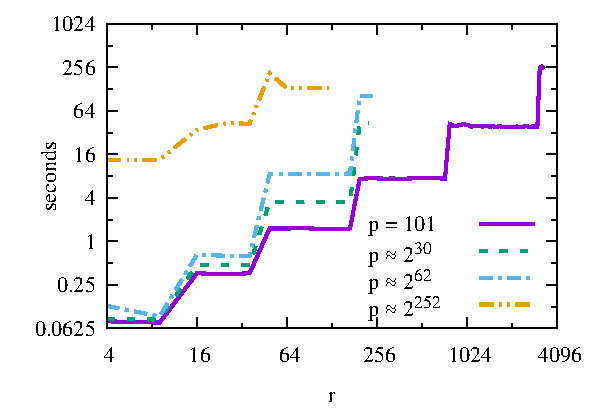
\includegraphics[scale=0.8]{Images/graphe-101-149-269.pdf}
\end{figure}
\end{frame}

%%%%%%%%%%%%%%%%%%%%%%%%%%%%%%%%%%%%%%%%%%%%%%%%%%%%%%%%%%%%

\begin{frame}
\frametitle{Conclusion}
\bluebox{Contribution}{
\begin{itemize}
\item A better understanding of the action of the Frobenius endomorphism on isogeny volcanoes. 

\item A faster variant of Couveignes' algorithm.

\end{itemize}
}
\bluebox{Future work}{
\begin{itemize}
\item Directly generalize to curves not on the crater.
\item Give an analogous algorithm for Atkin primes.
\end{itemize}}

%Code available on GitHub: \url{https://github.com/Hugounenq-Cyril/Two_curves_on_a_volcano}
\end{frame}

%%%%%%%%%%%%%%%%%%%%%%%%%%%%%%%%%%%%%%%%%%%%%%%%%%%%%%%%%%%%

\begin{frame} 

\bibliography{Biblio}
\end{frame}

\end{document}

%\begin{frame}
%%\frametitle{Going back to the initial curve}
%{
%%\begin{algorithmic}[1]
%%\STATE $\phi \leftarrow E \rightarrow E/\langle Q \rangle$
%%\STATE $P \leftarrow \phi(P)$
%%\RETURN $P$
%%\end{algorithmic}
%%\begin{algorithmic}[1]
%%\FOR{$i=1$ to $j-1$}
%%\STATE $(P,Q) \leftarrow \textbf{Rectify basis $ \left( P,Q \right)$}$ 
%%\STATE $\phi \leftarrow E \rightarrow E/\langle[2^{j-1}]Q\rangle$
%%\STATE $P \leftarrow \phi(P)$
%%\STATE $Q \leftarrow \phi(Q)/2$
%%\ENDFOR
%%\RETURN $P,Q$
%%\end{algorithmic}
%
%}
%
%\begin{columns}
%\begin{column}[c]{6cm}
%\begin{figure}[hbtp]
%\centering
%\includegraphics[scale=0.4]{Images/Volcan-go-left-premier.eps}
%\end{figure}
%
%\end{column}
%
%\begin{column}[c]{6cm}
%
%\begin{figure}[hbtp]
%\centering
%\includegraphics[scale=0.4]{Images/Volcan-go-left-deuxieme.eps}
%\end{figure}
%\end{column}
%
%\end{columns}
%\end{frame}
%
%
%\begin{frame}
%\begin{columns}
%\begin{column}[c]{6cm}
%\begin{figure}[hbtp]
%\centering
%\includegraphics[scale=0.4]{Images/Volcan-go-right-premier.eps}
%\end{figure}
%
%\end{column}
%
%\begin{column}[c]{6cm}
%
%\begin{figure}[hbtp]
%\centering
%\includegraphics[scale=0.4]{Images/Volcan-go-right-deuxieme.eps}
%\end{figure}
%
%\end{column}
%
%\end{columns}
%\end{frame}
%
%\begin{frame}
%\begin{figure}[hbtp]
%\centering
%\includegraphics[scale=0.8]{Images/Volcan-cratere-rouge-fleche-p-i.pdf} 
%\end{figure}
%\begin{rem}
%We need to give a direction to the horizontal isogeny we choose.
%\end{rem}
%\end{frame}
%
%\begin{frame}
%\bluebox{Benefit of the Frobenius}{
%We can distinguish two paths of length $k$ on the volcano one for each of the "eigenvalues" we have for the Frobenius endomorphism modulo $2^k$.
%}
%
%\begin{figure}[hbtp]
%\centering
%\includegraphics[scale=0.5]{Images/Volcan-cratere-rouge-fleche-lambda.pdf}
%\end{figure} 
%\begin{rem}
%We can always do that if the Frobenius is diagonalizable with two different "eigenvalues" denoted $\lambda_1, \lambda_2$.
%\end{rem}
%\end{frame}
%
%
%\begin{frame}
%\frametitle{Determination of a $2^k$ basis}
%\begin{figure}[hbtp]
%\centering
%\includegraphics[scale=0.4]{Images/Volcan-cratere-noir-chemin-rouge.pdf}
%\end{figure}
%
%\bluebox{Fact}{
%By determining a path of length $k$ on the crater we associate a set of points $P$ of order $2^k$ to this path. Because the path is associated to an $2^k$-isogeny then to the group generated by a primitive $2^k$ torsion point.} 
%\end{frame}
%
%
%\begin{frame}
%\section{Interpolation}
%\frametitle{Interpolation}
%\bluebox{}{
%We want to send point on $E$ that generates an horizontal isogeny associated to $\lambda_1$ on points on $E'$ that generates an horizontal isogeny associated to $\lambda_1$.
%\newline
%Thus we will have to interpolate points:
%\[
%P \rightarrow \mu P'$ with $\mu \wedge 2 =1
%\]
%\[
%Q \rightarrow \nu Q'$ with $\nu \wedge 2 =1
%\]
%}
%\end{frame}
%
%
%\begin{frame}
%\section{Determining a path on the cyclic crater}
%\frametitle{Curves on a cyclic crater}
%To take advantages of the Frobenius we go to an enough higher $2$-torsion where we have $2$ distinct "eigenvalues" for the Frobenius, we denote them by $\lambda_1, \lambda_2$.
%\newline
%\begin{defi}
%We denote by $k$ the least integer such that we have $\lambda_1 \neq \lambda_2 \bmod 2^k $
%\end{defi}
%\newline
%Thus we will work with $2^k$torsion points.
%\end{frame}
%
%
%\begin{frame}
%\frametitle{What about the isogenous curve?}
%\begin{figure}[hbtp]
%
%\centering
%\includegraphics[scale=0.4]{Images/duo-volcan-descendant-noir.pdf}
%\caption{Two volcanoes of $2$-isogeny of elliptic curves related by an odd isogeny}
%\end{figure}
%\end{frame}

%\begin{frame}
%\frametitle{How do we compute generators of the isogeny on the crater?}
%
%\bluebox{Compute $\langle P,Q \rangle = E[2^k]$}{
%\begin{algorithmic}[1]
%\REQUIRE $E: Y^2=X^3+A*X+B$
%\ENSURE $P, Q \in E$ such that $ \langle P,Q \rangle =E[2^k]$
%\end{algorithmic}}
%
%\bluebox{Rectify basis}
%{
%\begin{algorithmic}[1]
%\REQUIRE $\langle P,Q \rangle = E[2^k]$
%\ENSURE $P,Q$ such that $\pi(P)=\lambda_1P,$ $\pi(Q)=\lambda_2 Q, \langle P,Q \rangle = E[2^k]$
%\end{algorithmic}
%}
%\begin{figure}[hbtp]
%\centering
%\includegraphics[scale=0.25]{Images/Volcan-cratere-rectify.eps}
%\end{figure}
%
%
%\end{frame}


%\begin{frame}
%We work with a curve with the following type of $\ell$ structure:\[
%E(\mathbb{F}_q)[2^{\infty}]= \mathbb{Z}/2^{h}\mathbb{Z} \times \mathbb{Z}/2^{j}\mathbb{Z}
%\]with $h \geqslant j+1$
%
%$P$ and $Q$ two points such that : $E[2^{j+1}]=\langle P, Q \rangle$, with \textcolor{red}{$P \in E(\mathbb{F}_q), Q \notin E(\mathbb{F}_q)$}.
%
%\orangebox{Diagonal Matrix}{
%\[
%\pi(P,Q)=\left(\begin{array}{cc}
%1 & 0\\
%0 & q
%\end{array}\right) \bmod 2^{j+1}
%\]
%The points $Q$ associated to a diagonal matrix are the ones such that $\ell^{j}(Q)$ generates a unique $2$-isogeny.
%\newline
%This $2$-isogeny is horizontal if the volcano has a cyclic shaped crater.}
%
%\begin{rem}
%We work with parameters such that \textcolor{red}{$q \neq 1 \bmod 2^{j+1}$}
%\end{rem}
%\end{frame}


%\begin{frame}
%\frametitle{Going further on the crater}
%\begin{defi}[Desired basis]
%We denote by $T_2(E_i)$ the Tate module of $E_i$. We consider $\lambda_1 , \lambda_2$ the two "eigenvalues" of the Frobenius.
%We denote by \[P^i=(P^i_1,P^i_2,..), \pi(P_j^i)=\lambda_1 \cdot P_j^i, P_j^i=2 \cdot P_{j+1}^i \] such that $P_j^i$ is an $2^j$primitive torsion point on $E_i$. 
%We define the same way $Q^i=(Q^i_1,Q^i_2,...)$ with respect to $\lambda_2$.
%Thus we have $T_2(E_i)=(P^i,Q^i)$
%\end{defi}

%\bluebox{Basis intially known}
%{$\langle P_1^i,Q_1^i \rangle $is known with the Frobenius.
%Because we have $\pi(P_k^i)=\lambda_1P_k^1$ and also $\pi(P_k^i+Q_{k-1}^i)=\lambda_1(P_k^i+Q_{k-1}^i)$
%}
%\end{frame}

%\begin{frame}
%\frametitle{Recursive step}
%\begin{prop}
%If we know $Q_j^i \in E_i$ and a point $P \in E_i$ of order $2^k$ such that $\pi(P)=\lambda_1 P \neq \lambda_2 P$ then we are able to determine $Q_{j+1}^{i+1}$. 
%\end{prop}
%
%\begin{proof}
%We consider $\phi: E_i \rightarrow E_i/<2^{k-1}P_k^i>=E_{i+1}$. We have $Q_{j+1}^{i+1}=\phi(\frac{Q_j^i}{2}) $ since we can write  $\frac{Q_j^i}{2}= Q_{j+1}^{i}+ a  P_{1}^{i}$
%\end{proof}
%\end{frame}
